% Created by tikzDevice version 0.10.1 on 2016-11-22 07:08:50
% !TEX encoding = UTF-8 Unicode
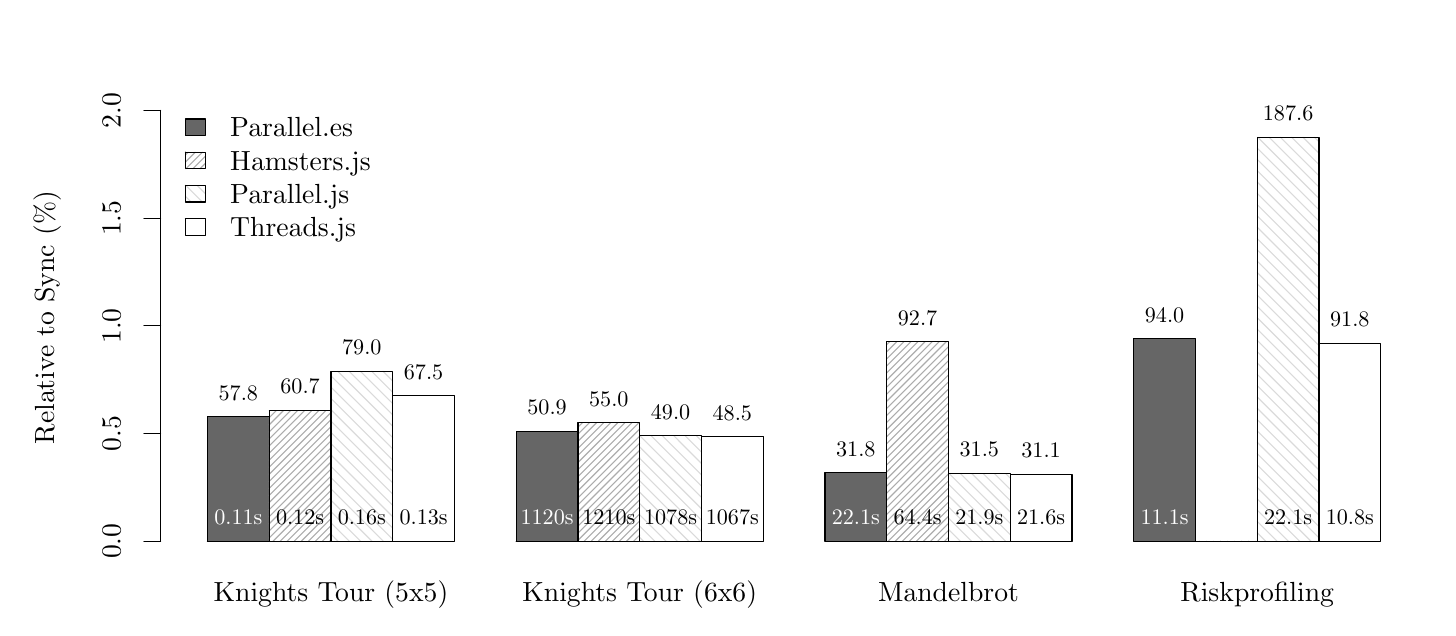
\begin{tikzpicture}[x=1pt,y=1pt]
\definecolor{fillColor}{RGB}{255,255,255}
\path[use as bounding box,fill=fillColor,fill opacity=0.00] (0,0) rectangle (505.89,209.58);
\begin{scope}
\path[clip] (  0.00,  0.00) rectangle (505.89,209.58);
\definecolor{fillColor}{gray}{0.40}

\path[fill=fillColor] ( 64.96, 24.00) --
	( 87.27, 24.00) --
	( 87.27, 68.96) --
	( 64.96, 68.96) --
	cycle;
\definecolor{drawColor}{RGB}{172,172,172}

\path[draw=drawColor,line width= 0.4pt,line join=round,line cap=round] ( 87.27, 71.18) -- ( 87.33, 71.24);

\path[draw=drawColor,line width= 0.4pt,line join=round,line cap=round] ( 87.27, 68.63) -- ( 89.88, 71.24);

\path[draw=drawColor,line width= 0.4pt,line join=round,line cap=round] ( 87.27, 66.07) -- ( 92.44, 71.24);

\path[draw=drawColor,line width= 0.4pt,line join=round,line cap=round] ( 87.27, 63.52) -- ( 94.99, 71.24);

\path[draw=drawColor,line width= 0.4pt,line join=round,line cap=round] ( 87.27, 60.96) -- ( 97.55, 71.24);

\path[draw=drawColor,line width= 0.4pt,line join=round,line cap=round] ( 87.27, 58.41) -- (100.10, 71.24);

\path[draw=drawColor,line width= 0.4pt,line join=round,line cap=round] ( 87.27, 55.85) -- (102.66, 71.24);

\path[draw=drawColor,line width= 0.4pt,line join=round,line cap=round] ( 87.27, 53.30) -- (105.21, 71.24);

\path[draw=drawColor,line width= 0.4pt,line join=round,line cap=round] ( 87.27, 50.74) -- (107.77, 71.24);

\path[draw=drawColor,line width= 0.4pt,line join=round,line cap=round] ( 87.27, 48.19) -- (109.59, 70.50);

\path[draw=drawColor,line width= 0.4pt,line join=round,line cap=round] ( 87.27, 45.63) -- (109.59, 67.95);

\path[draw=drawColor,line width= 0.4pt,line join=round,line cap=round] ( 87.27, 43.08) -- (109.59, 65.39);

\path[draw=drawColor,line width= 0.4pt,line join=round,line cap=round] ( 87.27, 40.52) -- (109.59, 62.84);

\path[draw=drawColor,line width= 0.4pt,line join=round,line cap=round] ( 87.27, 37.97) -- (109.59, 60.28);

\path[draw=drawColor,line width= 0.4pt,line join=round,line cap=round] ( 87.27, 35.41) -- (109.59, 57.73);

\path[draw=drawColor,line width= 0.4pt,line join=round,line cap=round] ( 87.27, 32.86) -- (109.59, 55.17);

\path[draw=drawColor,line width= 0.4pt,line join=round,line cap=round] ( 87.27, 30.30) -- (109.59, 52.62);

\path[draw=drawColor,line width= 0.4pt,line join=round,line cap=round] ( 87.27, 27.75) -- (109.59, 50.06);

\path[draw=drawColor,line width= 0.4pt,line join=round,line cap=round] ( 87.27, 25.19) -- (109.59, 47.51);

\path[draw=drawColor,line width= 0.4pt,line join=round,line cap=round] ( 88.64, 24.00) -- (109.59, 44.95);

\path[draw=drawColor,line width= 0.4pt,line join=round,line cap=round] ( 91.19, 24.00) -- (109.59, 42.40);

\path[draw=drawColor,line width= 0.4pt,line join=round,line cap=round] ( 93.75, 24.00) -- (109.59, 39.84);

\path[draw=drawColor,line width= 0.4pt,line join=round,line cap=round] ( 96.30, 24.00) -- (109.59, 37.29);

\path[draw=drawColor,line width= 0.4pt,line join=round,line cap=round] ( 98.86, 24.00) -- (109.59, 34.73);

\path[draw=drawColor,line width= 0.4pt,line join=round,line cap=round] (101.41, 24.00) -- (109.59, 32.17);

\path[draw=drawColor,line width= 0.4pt,line join=round,line cap=round] (103.97, 24.00) -- (109.59, 29.62);

\path[draw=drawColor,line width= 0.4pt,line join=round,line cap=round] (106.52, 24.00) -- (109.59, 27.06);

\path[draw=drawColor,line width= 0.4pt,line join=round,line cap=round] (109.08, 24.00) -- (109.59, 24.51);
\definecolor{drawColor}{RGB}{218,218,218}

\path[draw=drawColor,line width= 0.4pt,line join=round,line cap=round] (112.14, 24.00) -- (109.59, 26.56);

\path[draw=drawColor,line width= 0.4pt,line join=round,line cap=round] (116.23, 24.00) -- (109.59, 30.64);

\path[draw=drawColor,line width= 0.4pt,line join=round,line cap=round] (120.32, 24.00) -- (109.59, 34.73);

\path[draw=drawColor,line width= 0.4pt,line join=round,line cap=round] (124.41, 24.00) -- (109.59, 38.82);

\path[draw=drawColor,line width= 0.4pt,line join=round,line cap=round] (128.50, 24.00) -- (109.59, 42.91);

\path[draw=drawColor,line width= 0.4pt,line join=round,line cap=round] (131.90, 24.68) -- (109.59, 47.00);

\path[draw=drawColor,line width= 0.4pt,line join=round,line cap=round] (131.90, 28.77) -- (109.59, 51.09);

\path[draw=drawColor,line width= 0.4pt,line join=round,line cap=round] (131.90, 32.86) -- (109.59, 55.17);

\path[draw=drawColor,line width= 0.4pt,line join=round,line cap=round] (131.90, 36.95) -- (109.59, 59.26);

\path[draw=drawColor,line width= 0.4pt,line join=round,line cap=round] (131.90, 41.04) -- (109.59, 63.35);

\path[draw=drawColor,line width= 0.4pt,line join=round,line cap=round] (131.90, 45.12) -- (109.59, 67.44);

\path[draw=drawColor,line width= 0.4pt,line join=round,line cap=round] (131.90, 49.21) -- (109.59, 71.53);

\path[draw=drawColor,line width= 0.4pt,line join=round,line cap=round] (131.90, 53.30) -- (109.59, 75.62);

\path[draw=drawColor,line width= 0.4pt,line join=round,line cap=round] (131.90, 57.39) -- (109.59, 79.70);

\path[draw=drawColor,line width= 0.4pt,line join=round,line cap=round] (131.90, 61.48) -- (109.59, 83.79);

\path[draw=drawColor,line width= 0.4pt,line join=round,line cap=round] (131.90, 65.57) -- (112.03, 85.44);

\path[draw=drawColor,line width= 0.4pt,line join=round,line cap=round] (131.90, 69.65) -- (116.12, 85.44);

\path[draw=drawColor,line width= 0.4pt,line join=round,line cap=round] (131.90, 73.74) -- (120.20, 85.44);

\path[draw=drawColor,line width= 0.4pt,line join=round,line cap=round] (131.90, 77.83) -- (124.29, 85.44);

\path[draw=drawColor,line width= 0.4pt,line join=round,line cap=round] (131.90, 81.92) -- (128.38, 85.44);

\path[fill=fillColor] (176.53, 24.00) --
	(198.84, 24.00) --
	(198.84, 63.64) --
	(176.53, 63.64) --
	cycle;
\definecolor{drawColor}{RGB}{172,172,172}

\path[draw=drawColor,line width= 0.4pt,line join=round,line cap=round] (198.84, 65.22) -- (200.44, 66.82);

\path[draw=drawColor,line width= 0.4pt,line join=round,line cap=round] (198.84, 62.66) -- (203.00, 66.82);

\path[draw=drawColor,line width= 0.4pt,line join=round,line cap=round] (198.84, 60.11) -- (205.55, 66.82);

\path[draw=drawColor,line width= 0.4pt,line join=round,line cap=round] (198.84, 57.55) -- (208.11, 66.82);

\path[draw=drawColor,line width= 0.4pt,line join=round,line cap=round] (198.84, 55.00) -- (210.67, 66.82);

\path[draw=drawColor,line width= 0.4pt,line join=round,line cap=round] (198.84, 52.44) -- (213.22, 66.82);

\path[draw=drawColor,line width= 0.4pt,line join=round,line cap=round] (198.84, 49.89) -- (215.78, 66.82);

\path[draw=drawColor,line width= 0.4pt,line join=round,line cap=round] (198.84, 47.33) -- (218.33, 66.82);

\path[draw=drawColor,line width= 0.4pt,line join=round,line cap=round] (198.84, 44.78) -- (220.89, 66.82);

\path[draw=drawColor,line width= 0.4pt,line join=round,line cap=round] (198.84, 42.22) -- (221.16, 64.54);

\path[draw=drawColor,line width= 0.4pt,line join=round,line cap=round] (198.84, 39.67) -- (221.16, 61.98);

\path[draw=drawColor,line width= 0.4pt,line join=round,line cap=round] (198.84, 37.11) -- (221.16, 59.43);

\path[draw=drawColor,line width= 0.4pt,line join=round,line cap=round] (198.84, 34.56) -- (221.16, 56.87);

\path[draw=drawColor,line width= 0.4pt,line join=round,line cap=round] (198.84, 32.00) -- (221.16, 54.32);

\path[draw=drawColor,line width= 0.4pt,line join=round,line cap=round] (198.84, 29.45) -- (221.16, 51.76);

\path[draw=drawColor,line width= 0.4pt,line join=round,line cap=round] (198.84, 26.89) -- (221.16, 49.21);

\path[draw=drawColor,line width= 0.4pt,line join=round,line cap=round] (198.84, 24.34) -- (221.16, 46.65);

\path[draw=drawColor,line width= 0.4pt,line join=round,line cap=round] (201.06, 24.00) -- (221.16, 44.10);

\path[draw=drawColor,line width= 0.4pt,line join=round,line cap=round] (203.62, 24.00) -- (221.16, 41.54);

\path[draw=drawColor,line width= 0.4pt,line join=round,line cap=round] (206.17, 24.00) -- (221.16, 38.99);

\path[draw=drawColor,line width= 0.4pt,line join=round,line cap=round] (208.73, 24.00) -- (221.16, 36.43);

\path[draw=drawColor,line width= 0.4pt,line join=round,line cap=round] (211.28, 24.00) -- (221.16, 33.88);

\path[draw=drawColor,line width= 0.4pt,line join=round,line cap=round] (213.84, 24.00) -- (221.16, 31.32);

\path[draw=drawColor,line width= 0.4pt,line join=round,line cap=round] (216.39, 24.00) -- (221.16, 28.77);

\path[draw=drawColor,line width= 0.4pt,line join=round,line cap=round] (218.95, 24.00) -- (221.16, 26.21);
\definecolor{drawColor}{RGB}{218,218,218}

\path[draw=drawColor,line width= 0.4pt,line join=round,line cap=round] (222.53, 24.00) -- (221.16, 25.37);

\path[draw=drawColor,line width= 0.4pt,line join=round,line cap=round] (226.61, 24.00) -- (221.16, 29.45);

\path[draw=drawColor,line width= 0.4pt,line join=round,line cap=round] (230.70, 24.00) -- (221.16, 33.54);

\path[draw=drawColor,line width= 0.4pt,line join=round,line cap=round] (234.79, 24.00) -- (221.16, 37.63);

\path[draw=drawColor,line width= 0.4pt,line join=round,line cap=round] (238.88, 24.00) -- (221.16, 41.72);

\path[draw=drawColor,line width= 0.4pt,line join=round,line cap=round] (242.97, 24.00) -- (221.16, 45.81);

\path[draw=drawColor,line width= 0.4pt,line join=round,line cap=round] (243.47, 27.58) -- (221.16, 49.90);

\path[draw=drawColor,line width= 0.4pt,line join=round,line cap=round] (243.47, 31.67) -- (221.16, 53.98);

\path[draw=drawColor,line width= 0.4pt,line join=round,line cap=round] (243.47, 35.76) -- (221.16, 58.07);

\path[draw=drawColor,line width= 0.4pt,line join=round,line cap=round] (243.47, 39.85) -- (221.17, 62.15);

\path[draw=drawColor,line width= 0.4pt,line join=round,line cap=round] (243.47, 43.93) -- (225.26, 62.15);

\path[draw=drawColor,line width= 0.4pt,line join=round,line cap=round] (243.47, 48.02) -- (229.35, 62.15);

\path[draw=drawColor,line width= 0.4pt,line join=round,line cap=round] (243.47, 52.11) -- (233.44, 62.15);

\path[draw=drawColor,line width= 0.4pt,line join=round,line cap=round] (243.47, 56.20) -- (237.53, 62.15);

\path[draw=drawColor,line width= 0.4pt,line join=round,line cap=round] (243.47, 60.29) -- (241.61, 62.15);

\path[fill=fillColor] (288.10, 24.00) --
	(310.42, 24.00) --
	(310.42, 48.72) --
	(288.10, 48.72) --
	cycle;
\definecolor{drawColor}{RGB}{172,172,172}

\path[draw=drawColor,line width= 0.4pt,line join=round,line cap=round] (310.42, 95.03) -- (311.51, 96.12);

\path[draw=drawColor,line width= 0.4pt,line join=round,line cap=round] (310.42, 92.47) -- (314.06, 96.12);

\path[draw=drawColor,line width= 0.4pt,line join=round,line cap=round] (310.42, 89.92) -- (316.62, 96.12);

\path[draw=drawColor,line width= 0.4pt,line join=round,line cap=round] (310.42, 87.36) -- (319.17, 96.12);

\path[draw=drawColor,line width= 0.4pt,line join=round,line cap=round] (310.42, 84.81) -- (321.73, 96.12);

\path[draw=drawColor,line width= 0.4pt,line join=round,line cap=round] (310.42, 82.25) -- (324.28, 96.12);

\path[draw=drawColor,line width= 0.4pt,line join=round,line cap=round] (310.42, 79.70) -- (326.84, 96.12);

\path[draw=drawColor,line width= 0.4pt,line join=round,line cap=round] (310.42, 77.14) -- (329.39, 96.12);

\path[draw=drawColor,line width= 0.4pt,line join=round,line cap=round] (310.42, 74.59) -- (331.95, 96.12);

\path[draw=drawColor,line width= 0.4pt,line join=round,line cap=round] (310.42, 72.03) -- (332.73, 94.35);

\path[draw=drawColor,line width= 0.4pt,line join=round,line cap=round] (310.42, 69.48) -- (332.73, 91.79);

\path[draw=drawColor,line width= 0.4pt,line join=round,line cap=round] (310.42, 66.92) -- (332.73, 89.23);

\path[draw=drawColor,line width= 0.4pt,line join=round,line cap=round] (310.42, 64.37) -- (332.73, 86.68);

\path[draw=drawColor,line width= 0.4pt,line join=round,line cap=round] (310.42, 61.81) -- (332.73, 84.12);

\path[draw=drawColor,line width= 0.4pt,line join=round,line cap=round] (310.42, 59.26) -- (332.73, 81.57);

\path[draw=drawColor,line width= 0.4pt,line join=round,line cap=round] (310.42, 56.70) -- (332.73, 79.01);

\path[draw=drawColor,line width= 0.4pt,line join=round,line cap=round] (310.42, 54.14) -- (332.73, 76.46);

\path[draw=drawColor,line width= 0.4pt,line join=round,line cap=round] (310.42, 51.59) -- (332.73, 73.90);

\path[draw=drawColor,line width= 0.4pt,line join=round,line cap=round] (310.42, 49.03) -- (332.73, 71.35);

\path[draw=drawColor,line width= 0.4pt,line join=round,line cap=round] (310.42, 46.48) -- (332.73, 68.79);

\path[draw=drawColor,line width= 0.4pt,line join=round,line cap=round] (310.42, 43.92) -- (332.73, 66.24);

\path[draw=drawColor,line width= 0.4pt,line join=round,line cap=round] (310.42, 41.37) -- (332.73, 63.68);

\path[draw=drawColor,line width= 0.4pt,line join=round,line cap=round] (310.42, 38.81) -- (332.73, 61.13);

\path[draw=drawColor,line width= 0.4pt,line join=round,line cap=round] (310.42, 36.26) -- (332.73, 58.57);

\path[draw=drawColor,line width= 0.4pt,line join=round,line cap=round] (310.42, 33.70) -- (332.73, 56.02);

\path[draw=drawColor,line width= 0.4pt,line join=round,line cap=round] (310.42, 31.15) -- (332.73, 53.46);

\path[draw=drawColor,line width= 0.4pt,line join=round,line cap=round] (310.42, 28.59) -- (332.73, 50.91);

\path[draw=drawColor,line width= 0.4pt,line join=round,line cap=round] (310.42, 26.04) -- (332.73, 48.35);

\path[draw=drawColor,line width= 0.4pt,line join=round,line cap=round] (310.93, 24.00) -- (332.73, 45.80);

\path[draw=drawColor,line width= 0.4pt,line join=round,line cap=round] (313.49, 24.00) -- (332.73, 43.24);

\path[draw=drawColor,line width= 0.4pt,line join=round,line cap=round] (316.04, 24.00) -- (332.73, 40.69);

\path[draw=drawColor,line width= 0.4pt,line join=round,line cap=round] (318.60, 24.00) -- (332.73, 38.13);

\path[draw=drawColor,line width= 0.4pt,line join=round,line cap=round] (321.15, 24.00) -- (332.73, 35.58);

\path[draw=drawColor,line width= 0.4pt,line join=round,line cap=round] (323.71, 24.00) -- (332.73, 33.02);

\path[draw=drawColor,line width= 0.4pt,line join=round,line cap=round] (326.26, 24.00) -- (332.73, 30.47);

\path[draw=drawColor,line width= 0.4pt,line join=round,line cap=round] (328.82, 24.00) -- (332.73, 27.91);

\path[draw=drawColor,line width= 0.4pt,line join=round,line cap=round] (331.37, 24.00) -- (332.73, 25.36);
\definecolor{drawColor}{RGB}{218,218,218}

\path[draw=drawColor,line width= 0.4pt,line join=round,line cap=round] (332.91, 24.00) -- (332.73, 24.18);

\path[draw=drawColor,line width= 0.4pt,line join=round,line cap=round] (337.00, 24.00) -- (332.73, 28.26);

\path[draw=drawColor,line width= 0.4pt,line join=round,line cap=round] (341.08, 24.00) -- (332.73, 32.35);

\path[draw=drawColor,line width= 0.4pt,line join=round,line cap=round] (345.17, 24.00) -- (332.73, 36.44);

\path[draw=drawColor,line width= 0.4pt,line join=round,line cap=round] (349.26, 24.00) -- (332.73, 40.53);

\path[draw=drawColor,line width= 0.4pt,line join=round,line cap=round] (353.35, 24.00) -- (332.73, 44.62);

\path[draw=drawColor,line width= 0.4pt,line join=round,line cap=round] (355.05, 26.39) -- (332.94, 48.49);

\path[draw=drawColor,line width= 0.4pt,line join=round,line cap=round] (355.05, 30.48) -- (337.03, 48.49);

\path[draw=drawColor,line width= 0.4pt,line join=round,line cap=round] (355.05, 34.57) -- (341.12, 48.49);

\path[draw=drawColor,line width= 0.4pt,line join=round,line cap=round] (355.05, 38.66) -- (345.21, 48.49);

\path[draw=drawColor,line width= 0.4pt,line join=round,line cap=round] (355.05, 42.74) -- (349.30, 48.49);

\path[draw=drawColor,line width= 0.4pt,line join=round,line cap=round] (355.05, 46.83) -- (353.39, 48.49);

\path[fill=fillColor] (399.67, 24.00) --
	(421.99, 24.00) --
	(421.99, 97.18) --
	(399.67, 97.18) --
	cycle;
\definecolor{drawColor}{RGB}{172,172,172}

\path[draw=drawColor,line width= 0.4pt,line join=round,line cap=round] (423.36, 24.00) -- (423.36, 24.00);

\path[draw=drawColor,line width= 0.4pt,line join=round,line cap=round] (425.91, 24.00) -- (425.91, 24.00);

\path[draw=drawColor,line width= 0.4pt,line join=round,line cap=round] (428.47, 24.00) -- (428.47, 24.00);

\path[draw=drawColor,line width= 0.4pt,line join=round,line cap=round] (431.02, 24.00) -- (431.02, 24.00);

\path[draw=drawColor,line width= 0.4pt,line join=round,line cap=round] (433.58, 24.00) -- (433.58, 24.00);

\path[draw=drawColor,line width= 0.4pt,line join=round,line cap=round] (436.13, 24.00) -- (436.13, 24.00);

\path[draw=drawColor,line width= 0.4pt,line join=round,line cap=round] (438.69, 24.00) -- (438.69, 24.00);

\path[draw=drawColor,line width= 0.4pt,line join=round,line cap=round] (441.24, 24.00) -- (441.24, 24.00);

\path[draw=drawColor,line width= 0.4pt,line join=round,line cap=round] (443.80, 24.00) -- (443.80, 24.00);
\definecolor{drawColor}{RGB}{218,218,218}

\path[draw=drawColor,line width= 0.4pt,line join=round,line cap=round] (447.38, 24.00) -- (444.30, 27.07);

\path[draw=drawColor,line width= 0.4pt,line join=round,line cap=round] (451.47, 24.00) -- (444.30, 31.16);

\path[draw=drawColor,line width= 0.4pt,line join=round,line cap=round] (455.55, 24.00) -- (444.30, 35.25);

\path[draw=drawColor,line width= 0.4pt,line join=round,line cap=round] (459.64, 24.00) -- (444.30, 39.34);

\path[draw=drawColor,line width= 0.4pt,line join=round,line cap=round] (463.73, 24.00) -- (444.30, 43.43);

\path[draw=drawColor,line width= 0.4pt,line join=round,line cap=round] (466.62, 25.20) -- (444.30, 47.52);

\path[draw=drawColor,line width= 0.4pt,line join=round,line cap=round] (466.62, 29.29) -- (444.30, 51.60);

\path[draw=drawColor,line width= 0.4pt,line join=round,line cap=round] (466.62, 33.38) -- (444.30, 55.69);

\path[draw=drawColor,line width= 0.4pt,line join=round,line cap=round] (466.62, 37.47) -- (444.30, 59.78);

\path[draw=drawColor,line width= 0.4pt,line join=round,line cap=round] (466.62, 41.55) -- (444.30, 63.87);

\path[draw=drawColor,line width= 0.4pt,line join=round,line cap=round] (466.62, 45.64) -- (444.30, 67.96);

\path[draw=drawColor,line width= 0.4pt,line join=round,line cap=round] (466.62, 49.73) -- (444.30, 72.05);

\path[draw=drawColor,line width= 0.4pt,line join=round,line cap=round] (466.62, 53.82) -- (444.30, 76.13);

\path[draw=drawColor,line width= 0.4pt,line join=round,line cap=round] (466.62, 57.91) -- (444.30, 80.22);

\path[draw=drawColor,line width= 0.4pt,line join=round,line cap=round] (466.62, 62.00) -- (444.30, 84.31);

\path[draw=drawColor,line width= 0.4pt,line join=round,line cap=round] (466.62, 66.08) -- (444.30, 88.40);

\path[draw=drawColor,line width= 0.4pt,line join=round,line cap=round] (466.62, 70.17) -- (444.30, 92.49);

\path[draw=drawColor,line width= 0.4pt,line join=round,line cap=round] (466.62, 74.26) -- (444.30, 96.57);

\path[draw=drawColor,line width= 0.4pt,line join=round,line cap=round] (466.62, 78.35) -- (444.30,100.66);

\path[draw=drawColor,line width= 0.4pt,line join=round,line cap=round] (466.62, 82.44) -- (444.30,104.75);

\path[draw=drawColor,line width= 0.4pt,line join=round,line cap=round] (466.62, 86.52) -- (444.30,108.84);

\path[draw=drawColor,line width= 0.4pt,line join=round,line cap=round] (466.62, 90.61) -- (444.30,112.93);

\path[draw=drawColor,line width= 0.4pt,line join=round,line cap=round] (466.62, 94.70) -- (444.30,117.02);

\path[draw=drawColor,line width= 0.4pt,line join=round,line cap=round] (466.62, 98.79) -- (444.30,121.10);

\path[draw=drawColor,line width= 0.4pt,line join=round,line cap=round] (466.62,102.88) -- (444.30,125.19);

\path[draw=drawColor,line width= 0.4pt,line join=round,line cap=round] (466.62,106.97) -- (444.30,129.28);

\path[draw=drawColor,line width= 0.4pt,line join=round,line cap=round] (466.62,111.05) -- (444.30,133.37);

\path[draw=drawColor,line width= 0.4pt,line join=round,line cap=round] (466.62,115.14) -- (444.30,137.46);

\path[draw=drawColor,line width= 0.4pt,line join=round,line cap=round] (466.62,119.23) -- (444.30,141.54);

\path[draw=drawColor,line width= 0.4pt,line join=round,line cap=round] (466.62,123.32) -- (444.30,145.63);

\path[draw=drawColor,line width= 0.4pt,line join=round,line cap=round] (466.62,127.41) -- (444.30,149.72);

\path[draw=drawColor,line width= 0.4pt,line join=round,line cap=round] (466.62,131.49) -- (444.30,153.81);

\path[draw=drawColor,line width= 0.4pt,line join=round,line cap=round] (466.62,135.58) -- (444.30,157.90);

\path[draw=drawColor,line width= 0.4pt,line join=round,line cap=round] (466.62,139.67) -- (444.30,161.99);

\path[draw=drawColor,line width= 0.4pt,line join=round,line cap=round] (466.62,143.76) -- (444.30,166.07);

\path[draw=drawColor,line width= 0.4pt,line join=round,line cap=round] (466.62,147.85) -- (444.45,170.02);

\path[draw=drawColor,line width= 0.4pt,line join=round,line cap=round] (466.62,151.94) -- (448.53,170.02);

\path[draw=drawColor,line width= 0.4pt,line join=round,line cap=round] (466.62,156.02) -- (452.62,170.02);

\path[draw=drawColor,line width= 0.4pt,line join=round,line cap=round] (466.62,160.11) -- (456.71,170.02);

\path[draw=drawColor,line width= 0.4pt,line join=round,line cap=round] (466.62,164.20) -- (460.80,170.02);

\path[draw=drawColor,line width= 0.4pt,line join=round,line cap=round] (466.62,168.29) -- (464.89,170.02);
\definecolor{drawColor}{RGB}{0,0,0}

\path[draw=drawColor,line width= 0.4pt,line join=round,line cap=round] ( 64.96, 24.00) --
	( 87.27, 24.00) --
	( 87.27, 68.96) --
	( 64.96, 68.96) --
	( 64.96, 24.00);

\path[draw=drawColor,line width= 0.4pt,line join=round,line cap=round] ( 87.27, 24.00) --
	(109.59, 24.00) --
	(109.59, 71.24) --
	( 87.27, 71.24) --
	( 87.27, 24.00);

\path[draw=drawColor,line width= 0.4pt,line join=round,line cap=round] (109.59, 24.00) --
	(131.90, 24.00) --
	(131.90, 85.44) --
	(109.59, 85.44) --
	(109.59, 24.00);

\path[draw=drawColor,line width= 0.4pt,line join=round,line cap=round] (131.90, 24.00) --
	(154.22, 24.00) --
	(154.22, 76.52) --
	(131.90, 76.52) --
	(131.90, 24.00);

\path[draw=drawColor,line width= 0.4pt,line join=round,line cap=round] (176.53, 24.00) --
	(198.84, 24.00) --
	(198.84, 63.64) --
	(176.53, 63.64) --
	(176.53, 24.00);

\path[draw=drawColor,line width= 0.4pt,line join=round,line cap=round] (198.84, 24.00) --
	(221.16, 24.00) --
	(221.16, 66.82) --
	(198.84, 66.82) --
	(198.84, 24.00);

\path[draw=drawColor,line width= 0.4pt,line join=round,line cap=round] (221.16, 24.00) --
	(243.47, 24.00) --
	(243.47, 62.15) --
	(221.16, 62.15) --
	(221.16, 24.00);

\path[draw=drawColor,line width= 0.4pt,line join=round,line cap=round] (243.47, 24.00) --
	(265.79, 24.00) --
	(265.79, 61.77) --
	(243.47, 61.77) --
	(243.47, 24.00);

\path[draw=drawColor,line width= 0.4pt,line join=round,line cap=round] (288.10, 24.00) --
	(310.42, 24.00) --
	(310.42, 48.72) --
	(288.10, 48.72) --
	(288.10, 24.00);

\path[draw=drawColor,line width= 0.4pt,line join=round,line cap=round] (310.42, 24.00) --
	(332.73, 24.00) --
	(332.73, 96.12) --
	(310.42, 96.12) --
	(310.42, 24.00);

\path[draw=drawColor,line width= 0.4pt,line join=round,line cap=round] (332.73, 24.00) --
	(355.05, 24.00) --
	(355.05, 48.49) --
	(332.73, 48.49) --
	(332.73, 24.00);

\path[draw=drawColor,line width= 0.4pt,line join=round,line cap=round] (355.05, 24.00) --
	(377.36, 24.00) --
	(377.36, 48.19) --
	(355.05, 48.19) --
	(355.05, 24.00);

\path[draw=drawColor,line width= 0.4pt,line join=round,line cap=round] (399.67, 24.00) --
	(421.99, 24.00) --
	(421.99, 97.18) --
	(399.67, 97.18) --
	(399.67, 24.00);

\path[draw=drawColor,line width= 0.4pt,line join=round,line cap=round] (421.99, 24.00) --
	(444.30, 24.00) --
	(421.99, 24.00);

\path[draw=drawColor,line width= 0.4pt,line join=round,line cap=round] (444.30, 24.00) --
	(466.62, 24.00) --
	(466.62,170.02) --
	(444.30,170.02) --
	(444.30, 24.00);

\path[draw=drawColor,line width= 0.4pt,line join=round,line cap=round] (466.62, 24.00) --
	(488.93, 24.00) --
	(488.93, 95.47) --
	(466.62, 95.47) --
	(466.62, 24.00);
\end{scope}
\begin{scope}
\path[clip] (  0.00,  0.00) rectangle (505.89,209.58);
\definecolor{drawColor}{RGB}{0,0,0}

\node[text=drawColor,anchor=base,inner sep=0pt, outer sep=0pt, scale=  1.00] at (109.59,  2.40) {Knights Tour (5x5)};

\node[text=drawColor,anchor=base,inner sep=0pt, outer sep=0pt, scale=  1.00] at (221.16,  2.40) {Knights Tour (6x6)};

\node[text=drawColor,anchor=base,inner sep=0pt, outer sep=0pt, scale=  1.00] at (332.73,  2.40) {Mandelbrot};

\node[text=drawColor,anchor=base,inner sep=0pt, outer sep=0pt, scale=  1.00] at (444.30,  2.40) {Riskprofiling};
\end{scope}
\begin{scope}
\path[clip] (  0.00,  0.00) rectangle (505.89,209.58);
\definecolor{drawColor}{RGB}{0,0,0}

\node[text=drawColor,rotate= 90.00,anchor=base,inner sep=0pt, outer sep=0pt, scale=  1.00] at (  9.60,104.79) {Relative to Sync ({\%})};
\end{scope}
\begin{scope}
\path[clip] (  0.00,  0.00) rectangle (505.89,209.58);
\definecolor{drawColor}{RGB}{0,0,0}

\path[draw=drawColor,line width= 0.4pt,line join=round,line cap=round] ( 48.00, 24.00) -- ( 48.00,179.64);

\path[draw=drawColor,line width= 0.4pt,line join=round,line cap=round] ( 48.00, 24.00) -- ( 42.00, 24.00);

\path[draw=drawColor,line width= 0.4pt,line join=round,line cap=round] ( 48.00, 62.91) -- ( 42.00, 62.91);

\path[draw=drawColor,line width= 0.4pt,line join=round,line cap=round] ( 48.00,101.82) -- ( 42.00,101.82);

\path[draw=drawColor,line width= 0.4pt,line join=round,line cap=round] ( 48.00,140.73) -- ( 42.00,140.73);

\path[draw=drawColor,line width= 0.4pt,line join=round,line cap=round] ( 48.00,179.64) -- ( 42.00,179.64);

\node[text=drawColor,rotate= 90.00,anchor=base,inner sep=0pt, outer sep=0pt, scale=  1.00] at ( 33.60, 24.00) {0.0};

\node[text=drawColor,rotate= 90.00,anchor=base,inner sep=0pt, outer sep=0pt, scale=  1.00] at ( 33.60, 62.91) {0.5};

\node[text=drawColor,rotate= 90.00,anchor=base,inner sep=0pt, outer sep=0pt, scale=  1.00] at ( 33.60,101.82) {1.0};

\node[text=drawColor,rotate= 90.00,anchor=base,inner sep=0pt, outer sep=0pt, scale=  1.00] at ( 33.60,140.73) {1.5};

\node[text=drawColor,rotate= 90.00,anchor=base,inner sep=0pt, outer sep=0pt, scale=  1.00] at ( 33.60,179.64) {2.0};
\end{scope}
\begin{scope}
\path[clip] ( 48.00, 24.00) rectangle (505.89,185.58);
\definecolor{fillColor}{gray}{0.40}

\path[fill=fillColor] ( 57.00,176.58) --
	( 64.20,176.58) --
	( 64.20,170.58) --
	( 57.00,170.58) --
	cycle;
\definecolor{drawColor}{RGB}{172,172,172}

\path[draw=drawColor,line width= 0.4pt,line join=round,line cap=round] ( 57.00,163.56) -- ( 58.03,164.58);

\path[draw=drawColor,line width= 0.4pt,line join=round,line cap=round] ( 57.00,161.00) -- ( 60.58,164.58);

\path[draw=drawColor,line width= 0.4pt,line join=round,line cap=round] ( 57.14,158.58) -- ( 63.14,164.58);

\path[draw=drawColor,line width= 0.4pt,line join=round,line cap=round] ( 59.69,158.58) -- ( 64.20,163.09);

\path[draw=drawColor,line width= 0.4pt,line join=round,line cap=round] ( 62.25,158.58) -- ( 64.20,160.54);
\definecolor{drawColor}{RGB}{218,218,218}

\path[draw=drawColor,line width= 0.4pt,line join=round,line cap=round] ( 59.06,146.58) -- ( 57.00,148.64);

\path[draw=drawColor,line width= 0.4pt,line join=round,line cap=round] ( 63.15,146.58) -- ( 57.15,152.58);

\path[draw=drawColor,line width= 0.4pt,line join=round,line cap=round] ( 64.20,149.62) -- ( 61.24,152.58);
\definecolor{drawColor}{RGB}{0,0,0}

\path[draw=drawColor,line width= 0.4pt,line join=round,line cap=round] ( 57.00,176.58) --
	( 64.20,176.58) --
	( 64.20,170.58) --
	( 57.00,170.58) --
	( 57.00,176.58);

\path[draw=drawColor,line width= 0.4pt,line join=round,line cap=round] ( 57.00,164.58) --
	( 64.20,164.58) --
	( 64.20,158.58) --
	( 57.00,158.58) --
	( 57.00,164.58);

\path[draw=drawColor,line width= 0.4pt,line join=round,line cap=round] ( 57.00,152.58) --
	( 64.20,152.58) --
	( 64.20,146.58) --
	( 57.00,146.58) --
	( 57.00,152.58);

\path[draw=drawColor,line width= 0.4pt,line join=round,line cap=round] ( 57.00,140.58) --
	( 64.20,140.58) --
	( 64.20,134.58) --
	( 57.00,134.58) --
	( 57.00,140.58);

\node[text=drawColor,anchor=base west,inner sep=0pt, outer sep=0pt, scale=  1.00] at ( 73.20,170.14) {Parallel.es};

\node[text=drawColor,anchor=base west,inner sep=0pt, outer sep=0pt, scale=  1.00] at ( 73.20,158.14) {Hamsters.js};

\node[text=drawColor,anchor=base west,inner sep=0pt, outer sep=0pt, scale=  1.00] at ( 73.20,146.14) {Parallel.js};

\node[text=drawColor,anchor=base west,inner sep=0pt, outer sep=0pt, scale=  1.00] at ( 73.20,134.14) {Threads.js};

\node[text=drawColor,anchor=base,inner sep=0pt, outer sep=0pt, scale=  0.80] at ( 76.12, 74.96) {57.8};

\node[text=drawColor,anchor=base,inner sep=0pt, outer sep=0pt, scale=  0.80] at ( 98.43, 77.24) {60.7};

\node[text=drawColor,anchor=base,inner sep=0pt, outer sep=0pt, scale=  0.80] at (120.74, 91.44) {79.0};

\node[text=drawColor,anchor=base,inner sep=0pt, outer sep=0pt, scale=  0.80] at (143.06, 82.52) {67.5};

\node[text=drawColor,anchor=base,inner sep=0pt, outer sep=0pt, scale=  0.80] at (187.69, 69.64) {50.9};

\node[text=drawColor,anchor=base,inner sep=0pt, outer sep=0pt, scale=  0.80] at (210.00, 72.82) {55.0};

\node[text=drawColor,anchor=base,inner sep=0pt, outer sep=0pt, scale=  0.80] at (232.32, 68.15) {49.0};

\node[text=drawColor,anchor=base,inner sep=0pt, outer sep=0pt, scale=  0.80] at (254.63, 67.77) {48.5};

\node[text=drawColor,anchor=base,inner sep=0pt, outer sep=0pt, scale=  0.80] at (299.26, 54.72) {31.8};

\node[text=drawColor,anchor=base,inner sep=0pt, outer sep=0pt, scale=  0.80] at (321.57,102.12) {92.7};

\node[text=drawColor,anchor=base,inner sep=0pt, outer sep=0pt, scale=  0.80] at (343.89, 54.49) {31.5};

\node[text=drawColor,anchor=base,inner sep=0pt, outer sep=0pt, scale=  0.80] at (366.20, 54.19) {31.1};

\node[text=drawColor,anchor=base,inner sep=0pt, outer sep=0pt, scale=  0.80] at (410.83,103.18) {94.0};

\node[text=drawColor,anchor=base,inner sep=0pt, outer sep=0pt, scale=  0.80] at (455.46,176.02) {187.6};

\node[text=drawColor,anchor=base,inner sep=0pt, outer sep=0pt, scale=  0.80] at (477.77,101.47) {91.8};
\definecolor{drawColor}{RGB}{255,255,255}

\node[text=drawColor,anchor=base,inner sep=0pt, outer sep=0pt, scale=  0.80] at ( 76.12, 30.00) {0.11s};
\definecolor{drawColor}{RGB}{0,0,0}

\node[text=drawColor,anchor=base,inner sep=0pt, outer sep=0pt, scale=  0.80] at ( 98.43, 30.00) {0.12s};

\node[text=drawColor,anchor=base,inner sep=0pt, outer sep=0pt, scale=  0.80] at (120.74, 30.00) {0.16s};

\node[text=drawColor,anchor=base,inner sep=0pt, outer sep=0pt, scale=  0.80] at (143.06, 30.00) {0.13s};
\definecolor{drawColor}{RGB}{255,255,255}

\node[text=drawColor,anchor=base,inner sep=0pt, outer sep=0pt, scale=  0.80] at (187.69, 30.00) {1120s};
\definecolor{drawColor}{RGB}{0,0,0}

\node[text=drawColor,anchor=base,inner sep=0pt, outer sep=0pt, scale=  0.80] at (210.00, 30.00) {1210s};

\node[text=drawColor,anchor=base,inner sep=0pt, outer sep=0pt, scale=  0.80] at (232.32, 30.00) {1078s};

\node[text=drawColor,anchor=base,inner sep=0pt, outer sep=0pt, scale=  0.80] at (254.63, 30.00) {1067s};
\definecolor{drawColor}{RGB}{255,255,255}

\node[text=drawColor,anchor=base,inner sep=0pt, outer sep=0pt, scale=  0.80] at (299.26, 30.00) {22.1s};
\definecolor{drawColor}{RGB}{0,0,0}

\node[text=drawColor,anchor=base,inner sep=0pt, outer sep=0pt, scale=  0.80] at (321.57, 30.00) {64.4s};

\node[text=drawColor,anchor=base,inner sep=0pt, outer sep=0pt, scale=  0.80] at (343.89, 30.00) {21.9s};

\node[text=drawColor,anchor=base,inner sep=0pt, outer sep=0pt, scale=  0.80] at (366.20, 30.00) {21.6s};
\definecolor{drawColor}{RGB}{255,255,255}

\node[text=drawColor,anchor=base,inner sep=0pt, outer sep=0pt, scale=  0.80] at (410.83, 30.00) {11.1s};
\definecolor{drawColor}{RGB}{0,0,0}

\node[text=drawColor,anchor=base,inner sep=0pt, outer sep=0pt, scale=  0.80] at (455.46, 30.00) {22.1s};

\node[text=drawColor,anchor=base,inner sep=0pt, outer sep=0pt, scale=  0.80] at (477.77, 30.00) {10.8s};
\end{scope}
\end{tikzpicture}
